\documentclass{article}

\usepackage{graphicx}
\usepackage{tikz}
\usepackage{tikzsymbols}
\usetikzlibrary{calc,patterns,shapes.geometric}
\pagestyle{empty}
\usepackage[margin=0pt]{geometry}
\geometry{papersize={14in,12in}}

\def\centerarc[#1](#2)(#3:#4:#5){\draw[#1] ($(#2)+({#5*cos(#3)},{#5*sin(#3)})$) arc (#3:#4:#5);}

\begin{document}
	\begin{figure}
		\centering
		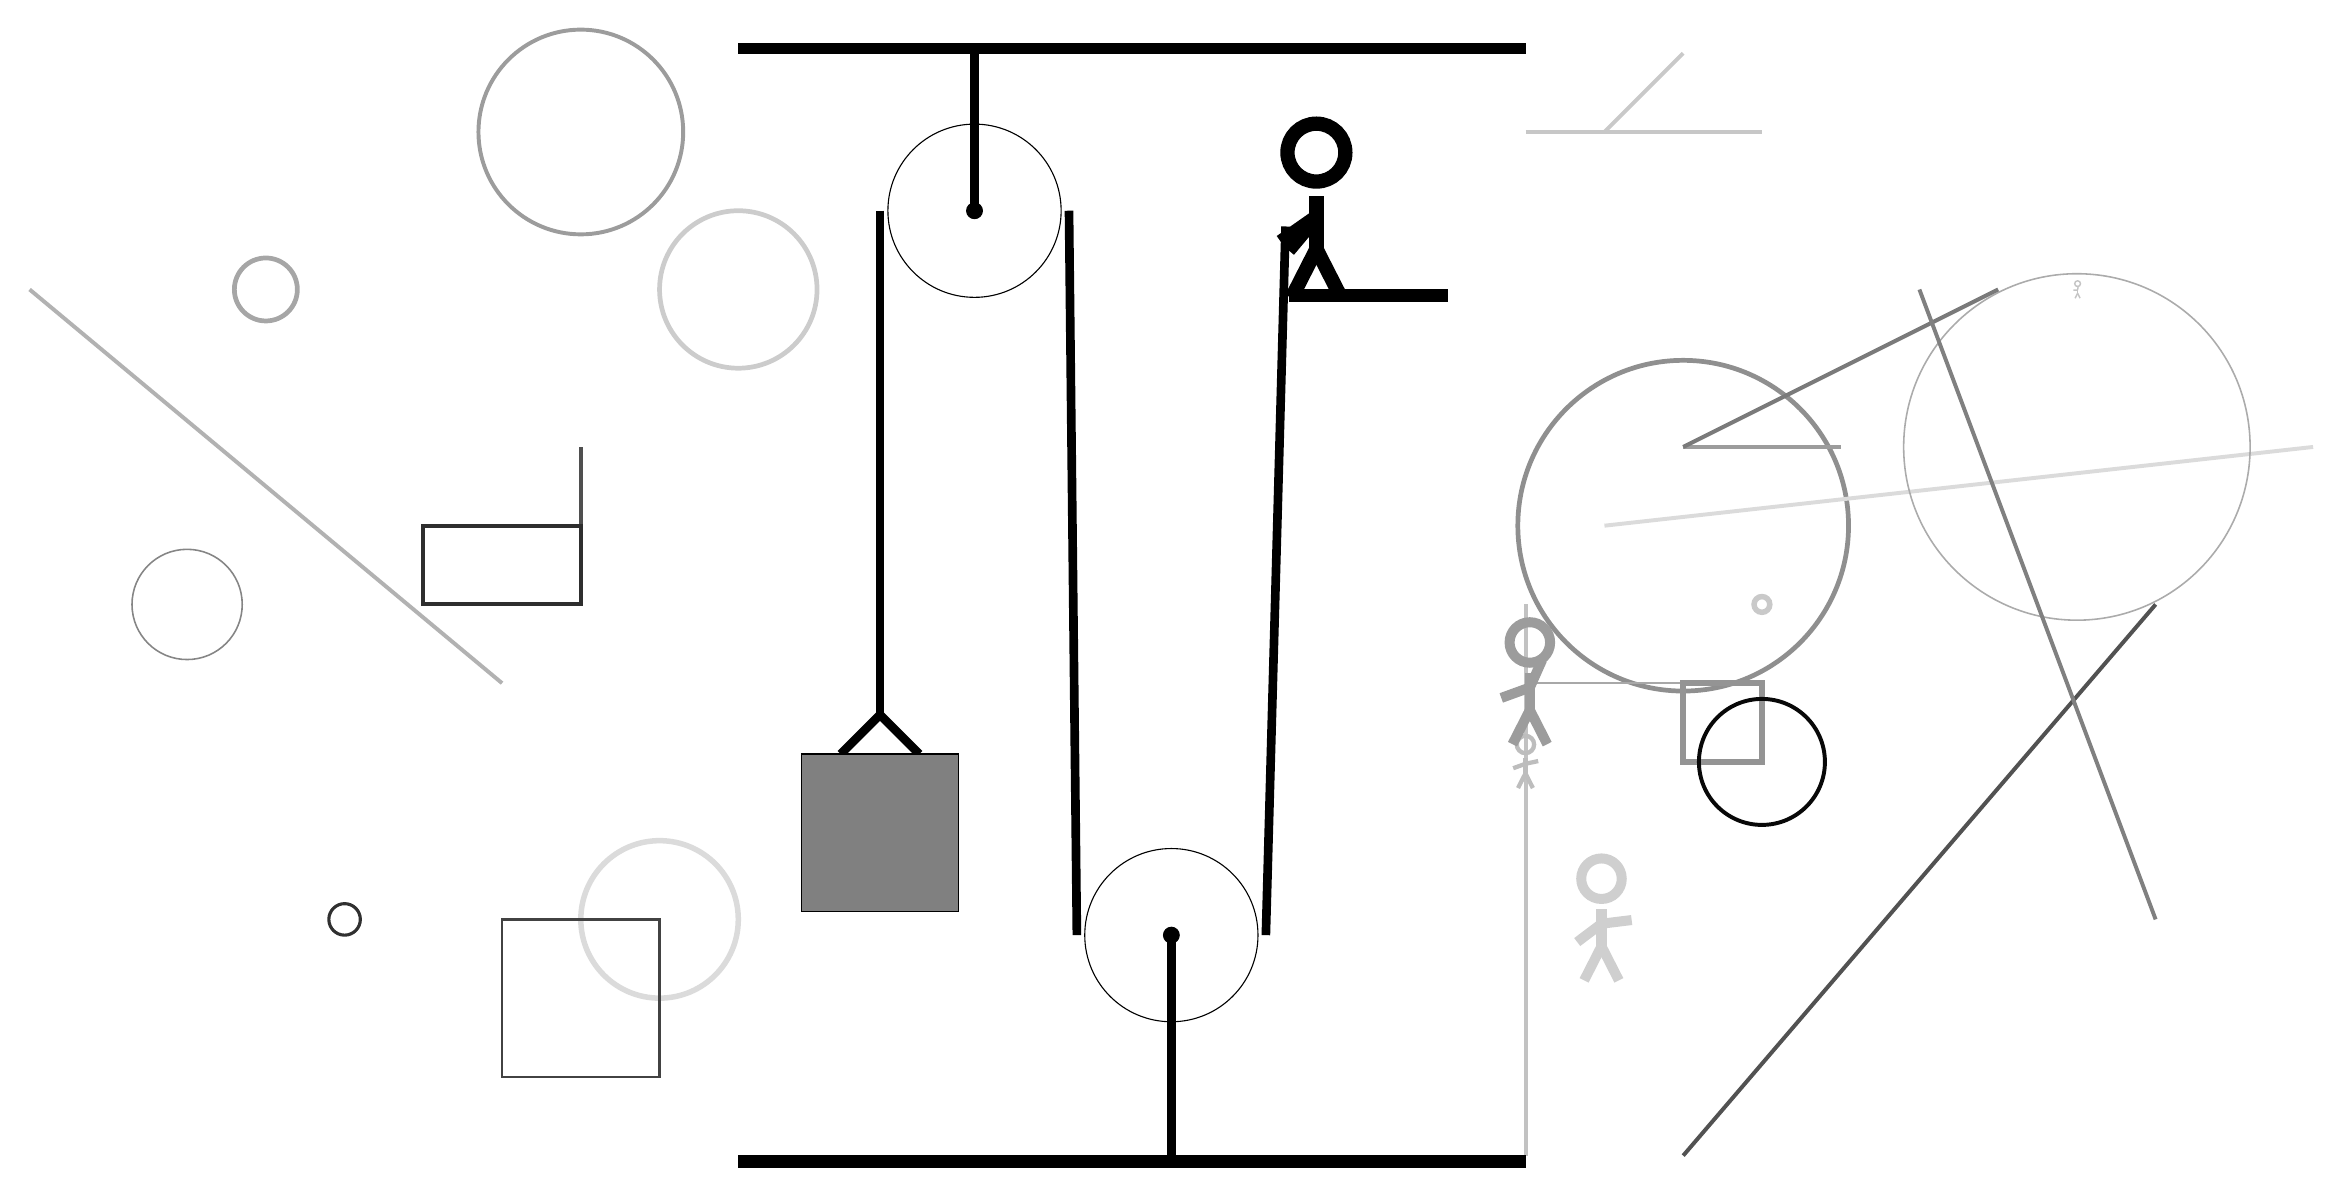
\begin{tikzpicture}
			%%%%% START %%%%%
			
			\draw[fill=black] (-2, 14) rectangle (8, 14.125);
			
			\draw (3.5, 2.8) circle (1.1);
			\draw[fill=black] (3.5, 2.8) circle (0.1);
			\draw[line width=1.1mm] (3.5, 2.8) -- (3.5, 0);
			
			\draw (1, 12) circle (1.1);
			\draw[fill=black] (1, 12) circle (0.1);
			\draw[line width=1.1mm] (1, 14) -- (1, 12);
			
			\draw [line width=0.7mm, color=black!14](-3, 3) circle (1.0);
			
			\draw [line width=0.6mm, color=black!44](10, 8) circle (2.1);
			\draw[line width=0.5mm, color=black!14](9, 8) -- (18, 9);
			\draw [line width=0.5mm, color=black!39](-4, 13) circle (1.3);
			\draw[line width=0.5mm, color=black!21](10, 14) -- (9, 13);
			\draw[line width=0.5mm, color=black!22](8, 13) -- (11, 13);
			
			\draw[line width=0.5mm, color=black!39](10, 9) -- (12, 9);
			\draw[line width=0.5mm, color=black!68](10, 0) -- (16, 7);
			\draw [line width=0.2mm, color=black!33](15, 9) circle (2.2);
			\node[line width=0.5mm, color=black!19] at (9, 3) {\Strichmaxerl[7][37][7]};
			\draw[line width=0.5mm, color=black!24](8, 0) -- (8, 7);
			
			\draw[line width=0.5mm, color=black!52](10, 9) -- (14, 11);
			\draw[line width=0.5mm, color=black!69](-4, 8) -- (-4, 9);
			
			\node[line width=0.2mm, color=black!26] at (8, 5) {\Strichmaxerl[3][20][12]};
			\draw [line width=0.7mm, color=black!63](-6, 6) circle (0.0);
			\draw[line width=0.3mm, color=black!34] (8, 6) rectangle (11, 6);
			
			\draw [line width=0.4mm, color=black!81](-7, 3) circle (0.2);
			
			\draw [line width=0.6mm, color=black!20](-2, 11) circle (1.0);
			\draw[line width=0.7mm, color=black!42] (10, 5) rectangle (11, 6);
			\draw[line width=0.5mm, color=black!50](13, 11) -- (16, 3);
			\draw[line width=0.5mm, color=black!82] (-4, 8) rectangle (-6, 7);
			\draw [line width=0.5mm, color=black!97](11, 5) circle (0.8);
			
			\draw[line width=0.3mm, color=black!74] (-3, 1) rectangle (-5, 3);
			\draw [line width=0.6mm, color=black!40](14, 7) circle (0.0);
			\node[line width=0.6mm, color=black!23] at (15, 11) {\Strichmaxerl[1][1][82]};
			
			\draw [line width=0.6mm, color=black!35](-8, 11) circle (0.4);
			\draw [line width=0.2mm, color=black!48](-9, 7) circle (0.7);
			\node[line width=0.4mm, color=black!39] at (8, 6) {\Strichmaxerl[7][20][66]};
			
			\draw[line width=0.5mm, color=black!30](-5, 6) -- (-11, 11);
			
			\draw [line width=0.7mm, color=black!21](11, 7) circle (0.1);
			
			\draw[line width=1.1mm](-0.7, 5.1) --  (-0.2, 5.6) -- (0.3, 5.1);
			\draw[fill=black!50] (-1.2, 5.1) rectangle (0.8, 3.1);
			
			\draw[line width=1.1mm](-0.2, 12) -- (-0.2, 5.6);
			\centerarc[line width=1.1mm](1, 12)(180:0:1.2000000000000002)
			\draw[line width=1.1mm](2.2, 12) -- (2.3, 2.8);
			\centerarc[line width=1.1mm](3.5, 2.8)(180:360:1.2000000000000002)
			\draw[line width=1.1mm](4.7, 2.8) -- (4.95, 11.8);
			
			\node at (5.3, 12) {\Strichmaxerl[10][35][-130]};
			\draw[fill=black] (5, 11) rectangle (7, 10.85);
			
			\draw[fill=black] (-2, 0) rectangle (8, -0.15);
			
			%%%%% END %%%%%
		\end{tikzpicture}
	\end{figure}	
\end{document}